\chapter{Problemanalyse}
\textit{I dette kapitel analyses problemstillinger, som opstår i forbindelse med lægemiddelskift. Disse problemstillinger vil sammenfattes i en opsummering og afsluttes med en problemformulering, der fremadrettet danner  grundlaget for rapporten.}

\section{Lægemiddelskift}
Lægemiddelskift forekommer når en ny lægemiddelvirksomhed vinder leverancen af nyt lægemiddel som standardbehandling, hvormed der er indgås et kontraktskift~\citep{Amgros2015}. 

Forinden et kontraktskift kan forekomme analyseres og vurderes lægemidlet i samarbejde med Medicinrådet og Amgros~\citep{DanskeRegioner2016}, som beskrevet i Appendiks \ref{cha:AppA}. Efter analyseringen og vurdering sendes lægemidlerne i udbud via Amgros med henblik på at indkøbe lægemidler af høj kvalitet til bedst mulige pris~\citep{Sygehusapoteket2017}.

Størstedelen af lægemidler i ATC-grupper sendes i udbud en gang årligt fra start september til midt november, hvor udbud på ATC-grupper som indgår i Medicinrådets behandlingsvejledninger sker løbende hen over året~\citep{Sygehusapoteket2017}, som beskrevet i Appendiks \ref{cha:AppD}.
Forinden udbuddet defineres antallet af vindere samt, hvorvidt udbuddet skal bygge på laveste pris eller være mest økonomisk fordelagtigt~\citep{Amgros2018a}, som beskrevet i Appendiks \ref{cha:AppB}.

På baggrund af de foregående analyser og vurderinger fastsættes et prisniveau der anvendes som beslutningsgrundlag for Medicinrådet om, hvorvidt lægemidlet skal anvendes som standardbehandling~\citep{DanskeRegioner2016}. Hvis standardbehandlingen er det eneste lægemiddel inden for terapiområdet kan dette implementeres direkte på hospitalet. I tilfælde af flere lægemidler inden for samme terapiområde, skal lægemidlernes ligeværdighed vurderes af Medicinrådet, som beskrevet i Appendiks \ref{cha:AppA}, med henblik på at udarbejde behandlingsvejledninger og rekommendationer for lægemidlerne. Disse videresendes til de danske hospitaler, som står for implementeringen.~\citep{DanskeRegioner2016}

Foruden kontraktskift kan lægemiddelskift forekomme, hvis efterspørgslen på et lægemiddel overstiger den tilgængelige mængde, hvormed der opstår restordre~\citep{Amgros2015}. Restordre kan f.eks. opstå ved leveringesvigt fra leverandøren eller producenten på det ønskede lægemiddel~\citep{Amgros2017, Laegemiddelinformaion2017}. Leveringesvigt skyldes som ofte at producenten har mangel på råvarer eller produktionsvanskeligheder~\citep{Amgros2017, Laegemiddelinformaion2017}. I tilfælde  af restordre er det leverandørens ansvar at dække sygehusapotekernes udgift ved indkøb af erstatningslægemiddel.~\citep{Laegemiddelinformaion2017, Amgros2017}

\section{Implementering af nyt lægemiddel}
Forinden et lægemiddel kan implementeres indkøbes lægemidlerne af Sygehusapoteket Region Nordjylland (SRN) som står for indkøb af lægemidler til distribution på de Nordjyske hospitaler ~\citep{SygehusapoteketRegionNordjylland2013}, som beskrevet i Appendiks \ref{cha:AppC}. Implementering af lægemidlet vurderes af ATC-ansvarlige, som er eksperter på området, som simpel eller kompleks på baggrund af flere faktorer~\citep{Sygehusapoteket2017}, som er beskrevet i Appendiks \ref{cha:AppD}. Dette indebærer f.eks. risikovurdering på afsnittet og lægemidlet samt type skift herunder bl.a. skift af dosis eller device og analoge lægemidler~\citep{Sygehusapoteket2017}. 

Et simpelt lægemiddelskift er vurderet til at påvirke klinikken i lav grad og varetages ofte af SRN's logistik afdeling~\citep{Laegemiddelinformaion2017, Sygehusapoteket2017a}. Disse skift sker dagligt i forbindelse med et simpel generisk lægemiddelskift. Hvorimod et kompleks lægemiddelskift påvirker klinikken i mellem til høj grad og kræver ofte involvering af flere interessenter som f.eks. medicinansvarlig, overlæger, kontaktsygeplejersker eller medicinservicefarmakonomer til at undersøge lægemidlets anvendelighed for det pågældende hospitalsafsnit. 
De komplekse skift sker ved generiske lægemidler, hvor flere faktorer som f.eks. styrke og disponeringsform afviger fra den nuværende behandling.~\citep{Laegemiddelinformaion2017,Sygehusapoteket2017a}

\section{Problemstillinger ved lægemiddelskift}
%Lægemiddelskift medvirker til reportering af utilsigtede hændelser (UTH'er)~\citep{Amgros2015}.
De hyppigste årsager til UTH'er på de danske hospitaler skyldes i år 2013 medicinering, hvilket udgjorde 23,97~\%.~\citep{Patientombuddet2013}. Antallet af rapporterede UTH'er i Region Nordjylland er steget med over 36\% fra år 2012 til 2014 ~\citep{Jensen2014}. Ud af 824 rapporterede UTH'er i år 2014 omhandlede 97\% af disse medicinering, 86\% administration af medicin og 41\% disponering~\citep{Jensen2014}. Det er i flere studier undersøgt de utilsigtede hændelser forårsaget af henholdsvis ordinationer, dispensering og administration af medicin, hvilket fremgår af tabel \ref{table:UTHordination}, \ref{table:UTHdispensering} og \ref{table:UTHAdministration}. En fælles årsag til de rapporterede UTH'er er forkert dosis, forkert lægemiddel og udeladelse af henholdsvis ordination, dispensering og administration.

	\vspace{2mm}
\begin{longtable}{p{5cm}|p{4.2cm}|p{2cm}|p{2cm}}
	\caption{Utilsigtede hændelser ved ordinationer.}
	\vspace{2mm}
	\label{table:UTHordination} \\
\cellcolor[HTML]{C0C0C0} {\textbf{Årsager}} & 
{\cellcolor[HTML]{C0C0C0}\textbf{Sundhedsstyrelsen~\citep{Sundhedsstyrelsen2005}}} &
{\cellcolor[HTML]{C0C0C0}\textbf{Lisby et al~\citep{Lisby2005}}} &
{\cellcolor[HTML]{C0C0C0}\textbf{Tully et al~\citep{Tully2009}}} \\ \hline
%{\cellcolor[HTML]{C0C0C0}\textbf{4}} 
%\textbf{Metode} & Gennemgang af indberettede UTH'er & Observation, stikprøvekontrol, journalgennemgang & Gennemgang af medicinlister & Gennemgang af indberettede UTH'er \\ \hline
Forkert dosis & - & - & 12,5~\%  \\ \hline %& 29,6      \\ \hline
Forkert lægemiddel & 16,3~\% & - & - \\ \hline % & 14,5 \\ \hline
Forkert patient & 3,8~\% & - & - \\ \hline %& 11,2 \\ \hline
Intet lægemiddel ordineret & 20,7~\% & - & 15,9~\% \\ \hline % & 24,1 \\ \hline
Udeladelse af formulering & - & 38,0~\% & - \\ \hline %& - \\ \hline
Udeladelse af administrationsvej & - & 34,7~\% & - \\ \hline %& - \\ \hline
Udeladelse af doseringstidspunkt & - & 10~\% & 10,4*~\% \\ \hline %& - \\ \hline
Manglende angivelse af maskimal dosis & - & - & 12,1~\% \\ \hline %& -  \\ \hline
Overset kontraindikation & 14,3~\% & - & 0,3~\% \\ \hline %& 19,6 \\ \hline
\cellcolor[HTML]{C0C0C0} {\textbf{Total antal fejl}} & 
{\cellcolor[HTML]{C0C0C0}\textbf{526}} &
{\cellcolor[HTML]{C0C0C0}\textbf{320}} &
{\cellcolor[HTML]{C0C0C0}\textbf{3455}}
\end{longtable}

Ud fra tabel \ref{table:UTHordination} fremgår det at de hyppigste årsager til UTH ved ordinationer skyldes 38~\% af de 320 rapportede UTH'er udeladelse af formulering og 34,7~\% administrationsvej~\citep{Lisby2005}. To studier påviste at i 20,7~\% ud af 526 og 15,9~\% af 3455 skyldes at intet lægemiddel var ordineret~\citep{Sundhedsstyrelsen2005, Tully2009}. Årsager som intet lægemiddel ordineret, udeladelse af doseringstidspunkt samt overset kontraindikation er dokumenteret af flere studier~\citep{Sundhedsstyrelsen2005, Lisby2005, Tully2009}. 

\vspace{2mm}
\begin{longtable}{p{5cm}|p{4.2cm}|p{2cm}|p{2cm}}
	\caption{Utilsigtede hændelser ved dispensering.}
	\vspace{2mm}
	\label{table:UTHdispensering} \\
\cellcolor[HTML]{C0C0C0} {\textbf{Årsager}} & 
{\cellcolor[HTML]{C0C0C0}\textbf{Sundhedsstyrelsen~\citep{Sundhedsstyrelsen2005}}} &
{\cellcolor[HTML]{C0C0C0}\textbf{Lisby et al~\citep{Lisby2005}}} &
{\cellcolor[HTML]{C0C0C0}\textbf{Barker et al~\citep{Barker2002}}} \\ \hline
%\textbf{Metode} & Gennemgang af indberettede UTH'er & Observation, stikprøvekontrol, journalgennemgang & Gennemgang af medicinlister & Gennemgang af indberettede UTH'er \\ \hline
Forkert dosis & 26,6~\% & 29,4~\% &  20,0~\% \\ \hline
Forkert lægemiddel & 52,2~\% & - & - \\ \hline
Forkert tidspunkt & - & 1,1~\% & 40,3~\% \\ \hline
Udeladt dispensering & 11,4~\% & 41,2~\% & 27,9~\% \\ \hline
%Dispensering af et
Ikke ordineret lægemiddel & - & 29,4 & 4,8 \\ \hline
\cellcolor[HTML]{C0C0C0} {\textbf{Total antal fejl}} & 
{\cellcolor[HTML]{C0C0C0}\textbf{184}} &
{\cellcolor[HTML]{C0C0C0}\textbf{17}} &
{\cellcolor[HTML]{C0C0C0}\textbf{290}}
\end{longtable}

Ud fra tabel \ref{table:UTHdispensering} fremgår det at de hyppigste årsager til UTH ved dispensering skyldes i 52,2~\% af de 184 rapporterede UTH'er forkert lægemiddel. Udover forkert lægemiddel blev der påvist forkert dosis, forkert tidspunkt eller udeladelse af dispensering samt ikke ordineret lægemiddel, hvor dette er dokumenteret i flere af studierne som værende en årsag til rapporteret UTH'er~\citep{Lisby2005, Sundhedsstyrelsen2005,Barker2002}.

\vspace{2mm}
\begin{longtable}{p{5cm}|p{4.2cm}|p{2cm}|p{2cm}}
	\caption{Utilsigtede hændelser ved administration.}
	\vspace{2mm}
	\label{table:UTHAdministration} \\
\cellcolor[HTML]{C0C0C0} {\textbf{Årsager}} & 
{\cellcolor[HTML]{C0C0C0}\textbf{Sundhedsstyrelsen~\citep{Sundhedsstyrelsen2005}}} &
{\cellcolor[HTML]{C0C0C0}\textbf{Lisby et al~\citep{Lisby2005}}} &
{\cellcolor[HTML]{C0C0C0}\textbf{Barker et al~\citep{Barker2002}}} \\ \hline
%\textbf{Metode} & Gennemgang af indberettede UTH'er & Observation, stikprøvekontrol, journalgennemgang & Gennemgang af medicinlister & Gennemgang af indberettede UTH'er \\ \hline
Forkert dosis & 37,5~\% & - & 20,0~\% \\ \hline
Forkert lægemiddel & 19,1~\% & - & - \\ \hline
Forkert tidspunkt & 8,9~\% & - & 40,3~\% \\ \hline
Forkert patient & - & 15,7~\% &  - \\ \hline
Udeladt administration & 15,0~\% & - & 27,9~\% \\ \hline
Manglende identifikation af patient & - & 78,9~\% & - \\ \hline
\cellcolor[HTML]{C0C0C0} {\textbf{Total antal fejl}} & 
{\cellcolor[HTML]{C0C0C0}\textbf{839}} &
{\cellcolor[HTML]{C0C0C0}\textbf{190}} &
{\cellcolor[HTML]{C0C0C0}\textbf{290}}
\end{longtable}
\vspace{0.25cm}

Ud fra tabel \ref{table:UTHAdministration} fremgår det at de hyppigste årsager til UTH ved administration i 78,9~\% af de 190 rapporterede UTH'er manglende patientidentifikation~\citep{Lisby2005}. I et af studierne skyldes 40,3~\% ud af 290 af tilfældene forkert tidspunkt~\citep{Barker2002} og i 37,5~\% af 839 forkert dosis~\citep{Sundhedsstyrelsen2005}. Forket dosis, forkert tidspunkt og udeladt administration var dokumenteret i flere studier~\citep{Lisby2005,Sundhedsstyrelsen2005,Barker2002}.

\subsection{Utilsigtede hændelser ved kontraktskift}
De patientsikkerhedsmæssige konsekvenser opstået ved kontraktskift er undersøgt af et norsk studie~\citep{Hakonsen2010}. Interview med 100 sygeplejersker påviste at der opstod fejlmedicinering ved generiske lægemidler. Fejl i ordination og manglende dokumentation af lægemiddelskift foretaget af lægen blev opdaget af 46~\% sygeplejersker dagligt, hvorimod sygeplejerskerne altid fik lægemiddelsiftet dokumenteret. Yderligere følte 92~\% af sygeplejerskerne at generiske lægemidler var tidskrævende og 91~\% at disse øgede risikoen for fejl ved disponering.~\citep{Hakonsen2010}. De typiske hændelser ved kontraktskift fremgår af Figur \ref{fig:UTHkontraktskift}.

\begin{figure}[H]\centering
	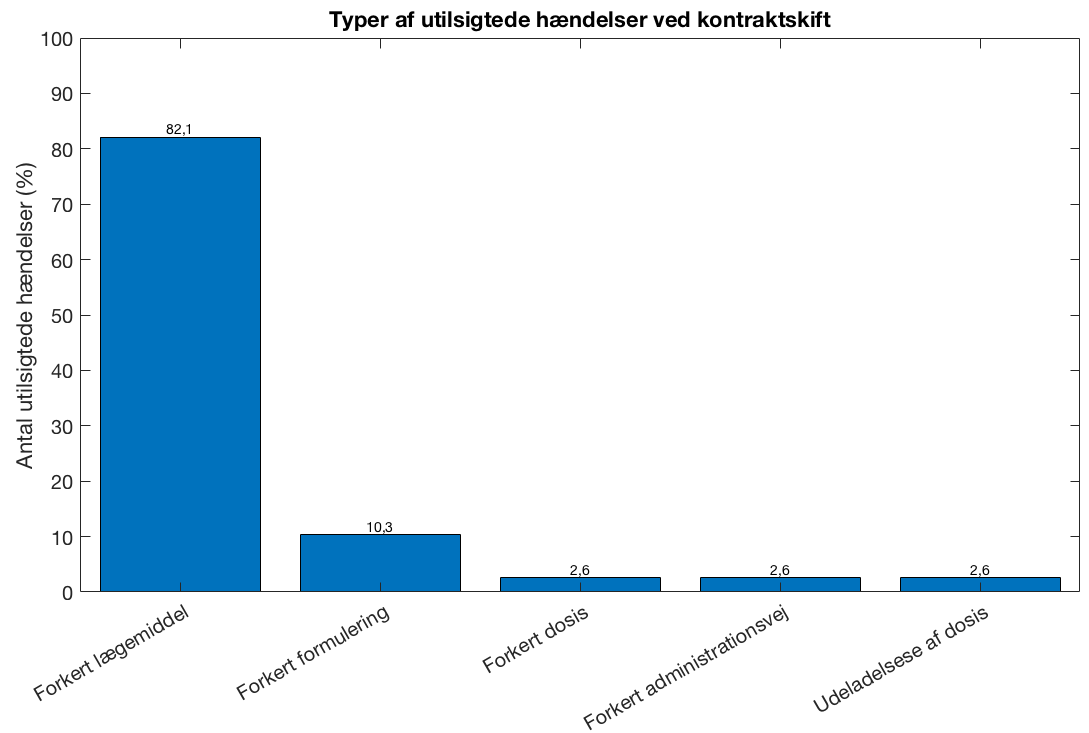
\includegraphics[width=1\textwidth]{billeder/UTH1.png} 
	\caption{Utilsigtede hændelser opstået ved kontraktskift\citep{Hakonsen2010}.}
	\label{fig:UTHkontraktskift}  
\end{figure}

Af Figur \ref{fig:UTHkontraktskift} fremgår det at 82,1~\% af UTH'erne forekommer ved disponering af forkert lægemiddel. Den næst hyppigste er forkert formulering hvor 10,3\% af UTH'er er berettiget mod dette. I  sjældnere tilfælde sker forkert dosis, administrationsvej samt udeladelse af dosis. 

\subsection{Utilsigtede hændelser ved restordre}
Studie har påvist at restordre påvirker patientsikkerheden ved anvendelse af generisk lægemiddel eller manglende alternativ behandling~\citep{Baumer2004}. Gennem spørgeskemaundersøgelse besvaret af farmaceuter blev UTH'er identificeret ved restordre. Undersøgelsen skelner mellem opståede hændelser og nærhændelser, som kunne være opstået~\citep{McLaughlin2013,McBride2013}. Typer af UTH'er identificeret ved restordre fremgår af figur \ref{fig:UTHrestordre}. 


\begin{figure}[H]\centering
	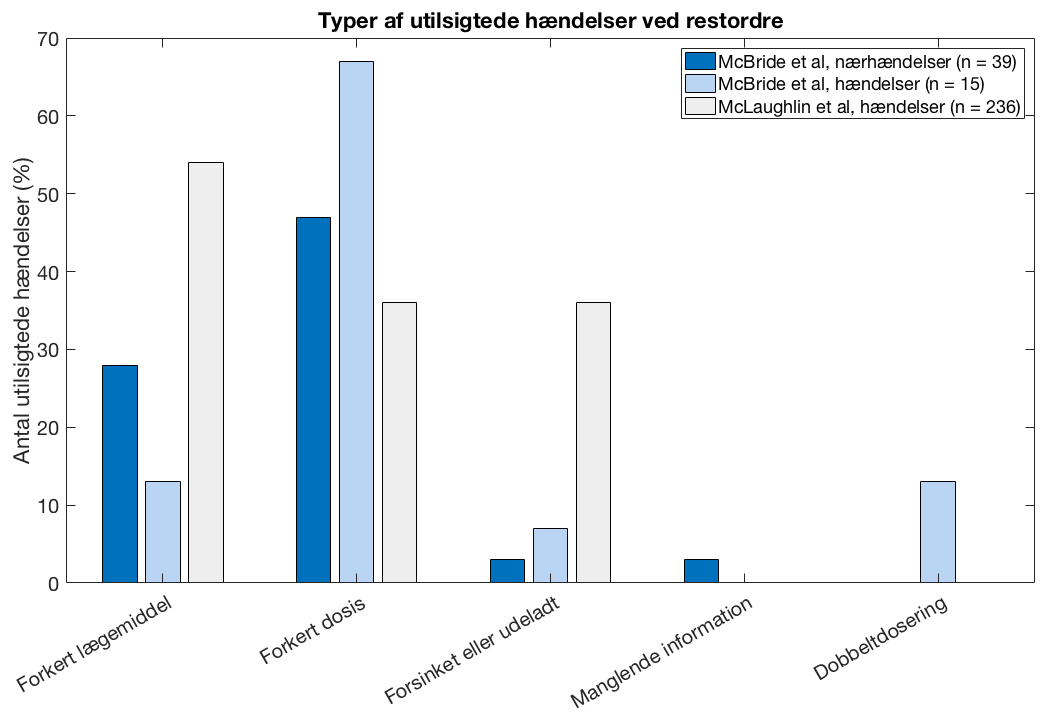
\includegraphics[width=1\textwidth]{billeder/UTH2.png} 
	\caption{Utilsigtede hændelser opstået ved restordre~\citep{McLaughlin2013,McBride2013}.}
	\label{fig:UTHrestordre}  
\end{figure}

Ud fra figur \ref{fig:UTHrestordre} fremgår det at forket dosis af lægemiddel og forsinket dosis var den hyppigste årsag til UTH'er ved restordre~\citep{McLaughlin2013,McBride2013}. Yderligere blev der i studierne identificeret UTH'er ved forsinket eller udeladt dispensering og administrering. Manglende information og dobbeltdosering blev påvist i et af studierne som en årsag til UTH'er ved restordre.~\citep{McLaughlin2013,McBride2013}

\section{Forebyggelse af problemstillinger ved lægemiddelskift}
De hyppigeste utilsigtede hændelser opstår i forbindelse med medicinering, administration og disponering~\citep{Jensen2014}. 
En måde at begrænse antallet af UTH'er er at synliggøre de problemstillinger der har medført rapporteringen af UTH'et. Ved at rapportere UTH'er kan de bagvedliggende årsager til fejl forebygges~\citep{StyrelsenforPatientsikkerhed2017}. Indbretningen af UTH'er er for sundhedsprofesionelle lovpligtigt~\citep{Jensen2014}. Yderligere blev det i år 2011 muligt for pårørende at rapportere UTH'er~\citep{Jensen2014}. På baggrund af rapporterede UTH'er er elektronisk patientmedicinering, stregkode scanning og klar-til-brug lægemidler implementeret med henblik på at nedbringe antallet af UTH'er.

\subsection{Elektronisk patientmedicinering}
Studier har påvist at implementering af elektronisk beslutningsstøtte reducerer antallet af UTH'er~\citep{DW1998,Bates2013,Cheng2011,Raboel2005} og beskrives som et vigtigt redskab til at øge kvaliteten af medicinering med henblik på at nedbringe fejl~\citep{Raboel2005}. I Danmark har indførsel af elektronisk patientmedicinering (EPM) medvirket til at reducere antallet af medicineringsfejl. Dette hjælper med at simplificere selve medicineringsprocessen, da dokumentation af ordination, dispensering og administration er samlet i ét system. Dette hjælpemiddel anvendes som et passivt beslutningsstøte for lægen ved ordination. Medicineringsfejl kan yderligere nedsættes hvis der udnyttes aktiv elektronisk beslutningsstøtte, hvor lægen vejledes f.eks. i forhold til lægemiddeldosis eller advares, hvis ordination kan være skadelig for patienten.~\citep{Raboel2005}. Til trods for at EPM har påvist at reducere antallet af UTH'er ved medicinering er der rapporteret UTH'er ved anvendelse af EPM~\citep{Syddanmark2008}, hvorfor der bør være fokus på forbedring og anvendelse af teknologier. 

%- Ny it-platform letter arbejdsgangene APOTO. APOTO skal levere data af høj kvalitet om lægemidler til sygehusenes EPJ systemer og på længere sigt kansystemet udvikles til også at under-støtte sygehusapotekernes produktion af lægemidler.  %[KILDE:Amgros_Årsmagasin2014, side 12]

\subsection{Stregkode scanning}
Internationale studier har påvist at stregkode scanning af lægemidler har en effekt på reducering af fejl i medicineringsprocessen~\citep{Poon2006,Bates2000,Levtzion-korach2010}. I Danmark anvender størstedelen af hospitalerne stregkode scanning, hvor lægemidlet kan spores fra leverandøren til patienten, hvilket medvirker til en effektiv lægemiddelforsyning og sikker medicinering ~\citep{Dzik2007,DPSD2008,Amgros2013}. Amgros har siden år 2010 stillet krav til stregkode på yderste og inderste emballage på lægemidler~\citep{Amgros2013}. Foruden at undgå alvorlige medicinrelaterede hændelser og reducere omkostninger samt tidsforbruget ved lagerstyring kan stregkoder medfører til andre positive resultater såsom, bedre sikring ved registering af lægemiddel i patienternes medicinjournal og effektiv tilbagekaldelse af medicin via it-systemer~\citep{Amgros2013}.
Implementering af stregkode scanning er påvirket af manglende stregkoder og dokumentation ved generisk lægemiddel. 

\subsection{Klar-til-brug lægemidler}
Internationale studier har påvist at automatisk dosisdispensering reducerer antallet af medicineringsfejl~\citep{Oren2003,Sygehusapotekerne2012}. I Danmark er der endnu ikke dokumenteret effekt på medicineringsfejl ved automatisk dosisdispensering, men påvist at reducering i fejl ved dispensering og administration~\citep{Sygehusapotekerne2012}. Dette er reduceret ved leveringen af klar-til-brug lægemidler såsom infusionsposer eller sprøjter, til de kliniske afdelinger~\citep{Sygehusapotekerne2012}. På denne måde skal personalet ikke tilberede lægemidlet, hvorved de skal håndtere farlige stoffer og det medvirker ligeledes til en sikre behandling for patienten, da risikoen for fejl er minimeret~\citep{Amgros2013}. 

\subsection{Vejledning}
*** Dette afsnit vil kunne lede godt op til det formål jeg har nemlig at kunne kategorisere sværhedsgraden af implementeringen med henblik på senere at kunne give vejledning til afdelingen på baggrund af denne ***

\section{Problemafgræsning}
På trods af at lægemidlerne sendes i udbud via Amgros med henblik på at opnå økonomiske besparelser er sundhedsudgifter til sygehusmedicin stigende. Udover det økonomiske aspekt medvirker implementeringen af lægemiddelskift til patientsikkerhedsmæssige konsekvenser. Dette bekræftes i det stigende antal af rapporterede UTH'er omhandlende medicinering herunder ordination, dispensering og administration. Flere løsninger er blevet anvendt i forhold til at reducere antallet af fejl ved medicinering herunder elektronisk beslutningsstøtte, stregkode scanning samt klar-til-brug.

*** Mangler en kobling til afsnittet under. Tænker at det kunne gøres ved at lave et afsnit omkring hvilken betydning vejledning har i forhold til at mindske fejl ***

På nuværende tidspunkt vurderes sværhedsgraden af implementeringen af lægemidler manuelt af en ATC-ansvarlig på SRN ud fra en skabelon, som fremgår af Appendiks \ref{cha:AppD}. Dette gør metoden sårbar da den er personafhængig, hvorfor et hjælpemiddel til at kategorisere sværhedsgraden ved implementeringen ønskes. 

\section{Problemformulering}
\textit{Hvilket potentiale har en algoritme til kategorisering af sværhedsgraden ved implementering af et nyt lægemiddel ud fra en række parametre der indsamles i forbindelse med Amgrosudbud?}
